\documentclass[11pt]{article}

\usepackage[a4paper,margin=2.2cm]{geometry}
\usepackage{amsmath}
\usepackage{graphicx}
\usepackage{float}
\usepackage{booktabs}
\usepackage{siunitx}
\usepackage[version=4]{mhchem}
\usepackage{chemfig}
\usepackage{hyperref}

\graphicspath{{figures/}}
\sisetup{per-mode=symbol, separate-uncertainty=true}

\title{Synthesis of Acetylsalicylic Acid (Aspirin)\\\large CHEM 2410 -- Organic Chemistry Laboratory}
\author{A.~Student \and Lab partner: B.~Partner}
\date{Experiment 4 -- 3 October 2026}

\begin{document}
\maketitle

\begin{abstract}
Acetylsalicylic acid was prepared by acid-catalysed acetylation of salicylic
acid with acetic anhydride. The crude product was recrystallised from
ethanol/water, giving white needles in \SI{71.4}{\percent} yield with a melting
point of \SIrange{134}{136}{\celsius}. Purity was assessed by TLC
(Figure~\ref{fig:tlc}) and the ferric chloride test.
\end{abstract}

\section{Introduction}
\label{sec:intro}

Aspirin (\ce{C9H8O4}) is synthesised by esterification of the phenolic hydroxyl
group of salicylic acid with acetic anhydride, using a few drops of concentrated
sulfuric acid as a catalyst~\cite{clayden2012,pavia2015}. The overall reaction is
shown in Equation~\eqref{eq:overall}:
\begin{equation}
  \ce{C7H6O3 + (CH3CO)2O ->[\ce{H2SO4}] C9H8O4 + CH3COOH}
  \label{eq:overall}
\end{equation}

The structure of the product is shown below.

\begin{center}
  \chemfig{*6((-COOH)=-=-=(-O-[::60]C(=[::60]O)-[::-60]CH_3)-)}
\end{center}

Excess acetic anhydride is destroyed during work-up by hydrolysis:
\ce{(CH3CO)2O + H2O -> 2 CH3COOH}. Unreacted salicylic acid gives a violet
complex with iron(III), \ce{Fe^3+ + 3 C7H5O3- -> [Fe(C7H5O3)3]}, which is the
basis of the purity test described in Section~\ref{sec:procedure}.

\section{Experimental Procedure}
\label{sec:procedure}

Salicylic acid (\SI{2.002}{\gram}, \SI{14.49}{\milli\mole}) was weighed into a
dry \SI{125}{\milli\litre} Erlenmeyer flask. Acetic anhydride
(\SI{5.0}{\milli\litre}, \SI{53}{\milli\mole}) and five drops of concentrated
\ce{H2SO4} were added, and the mixture was heated in a water bath at
\SI{85}{\celsius} for \SI{15}{\minute}.

After cooling, \SI{20}{\milli\litre} of ice-cold water was added to hydrolyse the
excess anhydride, and the flask was cooled in ice until crystallisation was
complete. The crude solid was collected by vacuum filtration
(Figure~\ref{fig:product}), washed with cold water, and recrystallised from
ethanol/water.

\begin{figure}[H]
  \centering
  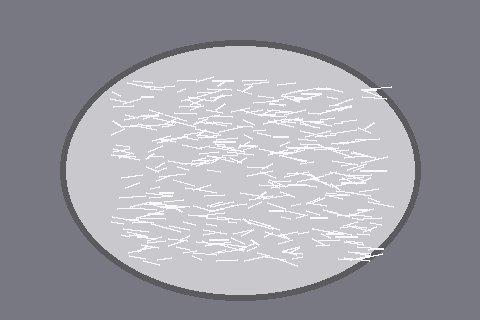
\includegraphics[width=0.55\textwidth]{product-photo.jpg}
  \caption{Recrystallised acetylsalicylic acid on the Büchner funnel.}
  \label{fig:product}
\end{figure}

\section{Results}
\label{sec:results}

The quantities used and the yield obtained are summarised in
Table~\ref{tab:yield}. The theoretical yield is based on salicylic acid as the
limiting reagent, with $M(\ce{C9H8O4}) = \SI{180.16}{\gram\per\mole}$:
\begin{equation}
  \text{yield} = \frac{m_\text{obs}}{n_\text{SA}\,M_\text{ASA}} \times 100
  = \frac{\SI{1.864}{\gram}}{\SI{14.49}{\milli\mole} \times \SI{180.16}{\gram\per\mole}}
  \times 100 = \SI{71.4}{\percent}
  \label{eq:yield}
\end{equation}

\begin{table}[H]
  \centering
  \caption{Reagents, product and yield.}
  \label{tab:yield}
  \begin{tabular}{l S[table-format=3.2] S[table-format=1.3] S[table-format=2.2]}
    \toprule
    {Compound} & {$M$ / \si{\gram\per\mole}} & {$m$ / \si{\gram}} & {$n$ / \si{\milli\mole}} \\
    \midrule
    Salicylic acid       & 138.12 & 2.002 & 14.49 \\
    Acetic anhydride     & 102.09 & 5.40  & 52.9  \\
    Aspirin (crude)      & 180.16 & 2.113 & 11.73 \\
    Aspirin (recryst.)   & 180.16 & 1.864 & 10.35 \\
    \bottomrule
  \end{tabular}
\end{table}

The TLC plate (silica, 1:1 ethyl acetate/hexane) is shown in
Figure~\ref{fig:tlc}. Retention factors were $R_f = 0.42$ for the product and
$R_f = 0.55$ for salicylic acid.

\begin{figure}[H]
  \centering
  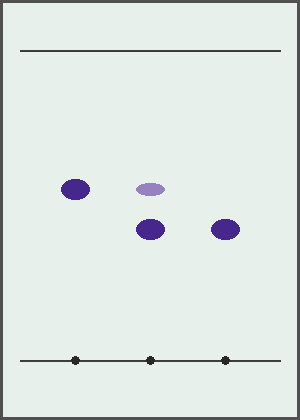
\includegraphics[width=0.4\textwidth]{tlc-plate.png}
  \caption{TLC plate under UV light: (1) salicylic acid, (2) crude product,
    (3) recrystallised product.}
  \label{fig:tlc}
\end{figure}

The measured melting point was \SIrange{134}{136}{\celsius} (literature
\SI{135}{\celsius}).

\section{Discussion}
\label{sec:discussion}

The yield of \SI{71.4}{\percent} (Equation~\ref{eq:yield}) is typical for this
experiment. Losses occurred mainly during recrystallisation, where some product
remained dissolved in the mother liquor. The narrow melting range and the single
spot on the TLC plate (Figure~\ref{fig:tlc}) indicate a pure product, which the
negative ferric chloride test confirms.

The crude product contained some unreacted salicylic acid, as shown by its
higher mass in Table~\ref{tab:yield} and a faint violet colour with
\ce{FeCl3}. Recrystallisation removed this impurity. Acetylation is effectively
irreversible under these conditions because the acetate leaving group,
\ce{CH3COO-}, is protonated in the acidic medium~\cite{clayden2012}.

\subsection{Conclusion}
Aspirin was prepared in good yield and high purity. The reaction mechanism and
the role of the acid catalyst were discussed in Section~\ref{sec:intro}.


\bibliographystyle{plain}
\bibliography{references}

\end{document}
